\documentclass[handout]{beamer}
\usepackage{docmute}
\usepackage[utf8]{inputenc}
\usepackage{hyperref}
\usepackage{forloop}
\usepackage{amsmath,amsfonts,amssymb}
\useoutertheme {smoothbars}
\usepackage{verbatim}
\usepackage{listings}
\usepackage{color}
\definecolor{name}{rgb}{0.5,0.5,0.5}
\definecolor{javared}{rgb}{0.6,0,0} % for strings
\definecolor{javagreen}{rgb}{0.25,0.5,0.35} % comments
\definecolor{javapurple}{rgb}{0.5,0,0.35} % keywords
\definecolor{javadocblue}{rgb}{0.25,0.35,0.75} % javadoc
\lstset{language=Java,
	basicstyle=\ttfamily,
	keywordstyle=\color{javapurple}\bfseries,
	stringstyle=\color{javared},
	commentstyle=\color{javagreen},
	morecomment=[s][\color{javadocblue}]{/**}{*/},
	numbers=left,
	numberstyle=\tiny\color{black},
	stepnumber=2,
	numbersep=10pt,
	tabsize=4,
	showspaces=false,
	showstringspaces=false}
\defbeamertemplate*{footline}{smoothbars theme}
{%
	\begin{beamercolorbox}[colsep=1.5pt]{upper separation line foot}
	\end{beamercolorbox}
	\begin{beamercolorbox}[ht=6ex,dp=1.125ex,%
		leftskip=.3cm,rightskip=.3cm plus1fil]{title in head/foot}%
		\leavevmode{\usebeamerfont{title in head/foot}\insertshorttitle}%
		\hfill%
		{\usebeamerfont{author in head/foot}\usebeamercolor[fg]{author in head/foot}\insertshortauthor}
		\vspace{.8mm}
		
		\url{http://creativecommons.org/licenses/by-nd/4.0/}%
	\end{beamercolorbox}%
	\begin{beamercolorbox}[colsep=1.5pt]{lower separation line foot}
	\end{beamercolorbox}
}
\author[Janis Streib]{Janis Streib \\ CC-BY-ND-4.0} 

\makeatletter
\AtBeginPart{%
	\beamer@tocsectionnumber=0\relax
	\setcounter{section}{0}
	%\def\pause{0}
	%\frame{\partpage}%
}
\makeatother

\begin{document}
	\part{Teil I}
	\documentclass{beamer}
\usepackage[utf8]{inputenc}
\usepackage{hyperref}
\usepackage{forloop}
\usepackage{amsmath,amsfonts,amssymb}
\useoutertheme {smoothbars}

\usepackage{listings}
\usepackage{color}
\definecolor{name}{rgb}{0.5,0.5,0.5}
\definecolor{javared}{rgb}{0.6,0,0} % for strings
\definecolor{javagreen}{rgb}{0.25,0.5,0.35} % comments
\definecolor{javapurple}{rgb}{0.5,0,0.35} % keywords
\definecolor{javadocblue}{rgb}{0.25,0.35,0.75} % javadoc
\lstset{language=Java,
	basicstyle=\ttfamily,
	keywordstyle=\color{javapurple}\bfseries,
	stringstyle=\color{javared},
	commentstyle=\color{javagreen},
	morecomment=[s][\color{javadocblue}]{/**}{*/},
	numbers=left,
	numberstyle=\tiny\color{black},
	stepnumber=2,
	numbersep=10pt,
	tabsize=4,
	showspaces=false,
	showstringspaces=false}
\defbeamertemplate*{footline}{smoothbars theme}
{%
	\begin{beamercolorbox}[colsep=1.5pt]{upper separation line foot}
	\end{beamercolorbox}
	\begin{beamercolorbox}[ht=6ex,dp=1.125ex,%
		leftskip=.3cm,rightskip=.3cm plus1fil]{title in head/foot}%
		\leavevmode{\usebeamerfont{title in head/foot}\insertshorttitle}%
		\hfill%
		{\usebeamerfont{author in head/foot}\usebeamercolor[fg]{author in head/foot}\insertshortauthor}
		\vspace{.8mm}
		
		\url{http://creativecommons.org/licenses/by-nd/4.0/}%
	\end{beamercolorbox}%
	\begin{beamercolorbox}[colsep=1.5pt]{lower separation line foot}
	\end{beamercolorbox}
}
\author[Janis Streib]{Janis Streib \\ CC-BY-ND-4.0} 

\begin{document}
%\def\pause{}
\title{RESTaurant for Android: Programmierung einer Sitzplatzreservierung \\ Teil I}   

\date{02.-06.11.2015} 

\frame{\titlepage} 

\frame{\frametitle{Inhalt}\tableofcontents} 

\section{JDK installieren}
\subsection{JDK}
\frame{\frametitle{JDK installieren}
 \begin{itemize}
 	\item Java Development Kit (JDK), der Compiler und Java Systembibliotheken enthält (aktuell: JDK8): \\
 	\url{https://www.oracle.com/technetwork/java/javase/downloads/jdk8-downloads-2133151.html}
\end{itemize}
}
\section{Android Studio installieren}
\subsection{Android Studio}
\frame{\frametitle{Android Studio installieren}
	\begin{itemize}
		\item Zur Gestaltung der späteren Benutzeroberfläche der App benötigen wir die offizielle Android-Entwicklungsumgebung
		\item Android Studio basiert auf der populären IDE IntelliJ
		\item Android Studio: \\
		\url{https://developer.android.com/sdk/index.html}
	\end{itemize}
}
\newcounter{ct}
\forloop{ct}{1}{\value{ct} < 9}%
{%
	\frame{\frametitle{Android Studio einrichten}		
			\includegraphics[width=116mm]{img/inst\arabic{ct}}	
	}
}

\section{NetBeans IDE installieren}
\subsection{NetBeans}
\frame{\frametitle{NetBeans IDE installieren}
	\begin{itemize}
		\item NetBeans IDE (for Java SE): \\
		\url{https://netbeans.org/}
		\item NBAndroid Plugin zur Androidentwicklung in NetBeans: \\
		\url{https://bitbucket.org/nbandroid/nbandroid/wiki/Installation}
		\item NetBeans Updatesite:
		\url{http://nbandroid.org/updates/updates.xml}
	\end{itemize}
}

\forloop{ct}{1}{\value{ct} < 11}%
{%
\frame{\frametitle{NetBeans IDE einrichten}		
		\includegraphics[width=116mm]{img/net\arabic{ct}}
}
}
\section{AVD einrichten}
	\frame{\frametitle{AVDs}		
		\begin{itemize}
			\item Das Android-SDK stellt die Möglichkeit eines Android-Emulators zur Verfügung
			\item Ermöglicht die Ausführung beliebiger Android-Versionen und Formfaktoren ohne echtes Smartphone/Tablet/Watch/...
			\item AVD := Android Virtual Device
		\end{itemize}
	}
\subsection{Image herunterladen}
\forloop{ct}{1}{\value{ct} < 3}%
{%
	\frame{\frametitle{Image herunterladen}		
		\includegraphics[width=116mm]{img/avd\arabic{ct}}
	}
}
\subsection{Virtuelles Smartphone einrichten}
\forloop{ct}{3}{\value{ct} < 9}%
{%
	\frame{\frametitle{Virtuelles Smartphone einrichten}		
		\includegraphics[width=116mm]{img/avd\arabic{ct}}
	}
}
\end{document}

   %  Load standalone SectionOne.tex
	\part{Teil II}
	\documentclass{beamer}
\usepackage[utf8]{inputenc}
\usepackage{hyperref}
\usepackage{forloop}
\usepackage{amsmath,amsfonts,amssymb}
\useoutertheme {smoothbars}

\usepackage{listings}

\usepackage{listings}
\usepackage{color}
\definecolor{name}{rgb}{0.5,0.5,0.5}
\definecolor{javared}{rgb}{0.6,0,0} % for strings
\definecolor{javagreen}{rgb}{0.25,0.5,0.35} % comments
\definecolor{javapurple}{rgb}{0.5,0,0.35} % keywords
\definecolor{javadocblue}{rgb}{0.25,0.35,0.75} % javadoc
\lstset{language=Java,
	basicstyle=\ttfamily,
	keywordstyle=\color{javapurple}\bfseries,
	stringstyle=\color{javared},
	commentstyle=\color{javagreen},
	morecomment=[s][\color{javadocblue}]{/**}{*/},
	numbers=left,
	numberstyle=\tiny\color{black},
	stepnumber=2,
	numbersep=10pt,
	tabsize=4,
	showspaces=false,
	showstringspaces=false}
\defbeamertemplate*{footline}{smoothbars theme}
{%
	\begin{beamercolorbox}[colsep=1.5pt]{upper separation line foot}
	\end{beamercolorbox}
	\begin{beamercolorbox}[ht=6ex,dp=1.125ex,%
		leftskip=.3cm,rightskip=.3cm plus1fil]{title in head/foot}%
		\leavevmode{\usebeamerfont{title in head/foot}\insertshorttitle}%
		\hfill%
		{\usebeamerfont{author in head/foot}\usebeamercolor[fg]{author in head/foot}\insertshortauthor}
		\vspace{.8mm}
		
		\url{http://creativecommons.org/licenses/by-nd/4.0/}%
	\end{beamercolorbox}%
	\begin{beamercolorbox}[colsep=1.5pt]{lower separation line foot}
	\end{beamercolorbox}
}
\author[Janis Streib]{Janis Streib \\ CC-BY-ND-4.0} 


\begin{document}
%\def\pause{}
\title{RESTaurant for Android: Programmierung einer Sitzplatzreservierung \\ Teil II}
\date{02.-06.11.2015} 

\frame{\titlepage} 

\frame{\frametitle{Inhalt}\tableofcontents} 

%\lstinputlisting{filename.java}
%\begin{lstlisting}
% Add code here
%\end{lstlisting}

\frame{\frametitle{Java in a Nutshell}		
	Was brauchen wir?
	\begin{itemize}
		\item Variablen
		\item Methoden
		\item Klassen
		\item $\Rightarrow$ Objektorientierung, Vererbung
		\item Kontrollstrukturen
		\item I/O (Eingabe/Ausgabe)/ Streams
		\item Exceptionhandling
		\item Generics
	\end{itemize}
}

\section{Kleine Aufgaben zum warm werden}
\subsection{Finde den Fehler!}
\frame{\frametitle{Finde den Fehler!}		
	\lstinputlisting{samples/Sample1.java}
}

\frame{\frametitle{Finde den Fehler!}		
	\begin{itemize}
		\item Kompiliert es? \pause
		\item $\Rightarrow$ \textcolor{red}{Nein}\pause
		\item Wie kann man es reparieren? \pause
		\item 'Hallo Welt!' ist ein String und muss deshalb in " "
		
	\end{itemize}
}

\frame{\frametitle{Finde den Fehler!}		
	\lstinputlisting{samples/Sample2.java}
}
\frame{\frametitle{Finde den Fehler!}		
	\begin{itemize}
		\item Kompiliert es? \pause
		\item $\Rightarrow$ \textcolor{green}{Ja}\pause
		\item Was ist die Ausgabe?\pause
		\item {\tt Error: Could not find or load main class Sample2} \pause
		\item Wie kann man es reparieren? \pause
		\item Die main-Methode muss immer statisch sein $\Rightarrow$ Codewort 'static'
		
	\end{itemize}
}

\frame{\frametitle{Finde den Fehler!}		
	\lstinputlisting{samples/Greeter.java}
}

\frame{\frametitle{Finde den Fehler!}		
	\begin{itemize}
		\item Kompiliert es? \pause
		\item $\Rightarrow$ \textcolor{red}{Nein}\pause
		\item Wie kann man es reparieren? \pause
		\item Eine neue Instanzvariable 'message' vom Typ String anlegen und im Konstruktor zuweisen.
		
	\end{itemize}
}

\frame{\frametitle{Finde den Fehler!}		
	\lstinputlisting{samples/Greeter2.java}
}

\frame{\frametitle{Finde den Fehler!}		
	\begin{itemize}
		\item Kompiliert es? \pause
		\item $\Rightarrow$ \textcolor{green}{Ja}\pause
		\item Was ist die Ausgabe?\pause
		\item {\tt null} \pause
		\item Wie kann man es reparieren? \pause
		\item Den Konstruktorparameter der Instanzvariable zuweisen (Codewort 'this', um auf die Instanz zuzugreifen anstatt der lokalen Variable)	
	\end{itemize}
}
\section{Generics}
\subsection{Beispiele}
\frame{\frametitle{Generics}
\begin{itemize}
	\item Zur Erzeugung generischer Objekte
	\item Beispiel: LinkedList$<\cdot>$, ArrayList$<\cdot>$, HashMap$<\cdot,\cdot>$, ...
	\item Audrücke wie "{\tt ? extends Object}" möglich, um auszudrücken, dass das Objekt "mindestens" ein bestimmtes Objekt zu sein hat (in der Vererbungshierarchie)
\end{itemize}	
}
\subsection{Implementierung/Benutzung}
\frame{\frametitle{Beispiel}
	Angenommen, man möchte eine LinkedList benutzen, um eine Menge von Kursteilnehmern zu speichern.
	Dazu bietet sich eine LinkedList an. Damit man in "unsere" LinkedList nur Objekte vom Typ "Kursteilnehmer" stecken kann, ist die LinkedList ein Generic.
	 \tiny {\lstinputlisting{samples/GenericSample.java}
	 \lstinputlisting{samples/Participant.java}}
}
\section{Objektorientierung}
\subsection{Modellierung}
\frame{\frametitle{Modellieren}		
	Modellieren Sie in Java: \\
	Ein \emph{Zug} ist entweder ein \emph{Personenzug} oder ein \emph{Güterzug}. Ein Zug hat genau eine \emph{Lokomotive}. Eine Lokomotive ist entweder ein \emph{elektrischer Triebwagen} oder ein \emph{Dieseltriebwagen}. Alle Lokomotiven können abhängig von ihrer Art eine \emph{Notbremsung} vollziehen. Ein Zug hat beliebig viele \emph{Wagons}. Dabei kann ein Personenzug aus \emph{Personenwagons} und \emph{Speisewagons} bestehen, ein Güterzug aus \emph{Containerwagons}. Alle genannten Bestandteile eines Zuges können \emph{gereinigt} werden (Wagons und Lokomotiven sind also \emph{"reinigbar"}).
}
\frame{\frametitle{Modellieren}		
	Welche Objekte ($\Leftrightarrow$ Klassen) sind \emph{abstrakt}? \pause
	\begin{itemize}
		\item Zug \pause
		\item Lokomotive \pause
		\item Wagon \pause
		\begin{itemize}
			\item Passagierwagen
			\item Güterwagon
		\end{itemize}
	\end{itemize}
}
\frame{\frametitle{Modellieren}		
	Welche Objekte ($\Leftrightarrow$ Klassen) sind \textcolor{green}{\emph{konkret}}? \pause
	\begin{itemize}
		\item Zug
		\begin{itemize}
			\item \textcolor{green}{Personenzug}
			\item \textcolor{green}{Güterzug}
		\end{itemize} \pause
		\item Lokomotive
		\begin{itemize}
			\item \textcolor{green}{Dieseltriebwagen}
			\item \textcolor{green}{Elektrischer Triebwagen}
		\end{itemize}
		\item Wagon
		\begin{itemize}
			\item Passagierwagon  \pause
			\begin{itemize}
				\item \textcolor{green}{Speisewagon}
				\item \textcolor{green}{Personenwagon}
			\end{itemize}
			\item Güterwagon \pause
			\begin{itemize}
				\item \textcolor{green}{Containerwagon}
			\end{itemize}
		\end{itemize}
	\end{itemize}
}
\frame{\frametitle{Implementieren!}
	\pause
	\tiny{
		\lstinputlisting[caption=Cleanable.java]{samples/Cleanable.java}
		 \lstinputlisting[caption=Locomotive.java]{samples/Locomotive.java}
		}
}
\frame{\frametitle{Implementieren!}
	\tiny{ 
		\lstinputlisting[caption=Bogie.java]{samples/Bogie.java}
		\lstinputlisting[caption=CargoBogie.java]{samples/CargoBogie.java}
		\lstinputlisting[caption=PassengerBogie.java]{samples/PassengerBogie.java}
	}
}
\frame{\frametitle{Implementieren!}
	\tiny{ 
		\lstinputlisting[caption=ElectricLocomotive.java]{samples/ElectricLocomotive.java}
	}
}
\frame{\frametitle{Implementieren!}
	\tiny{ 
		\lstinputlisting[caption=DieselLocomotive.java]{samples/DieselLocomotive.java}
	}
}
\frame{\frametitle{Implementieren!}
	\tiny{ 
	\lstinputlisting[caption=Train.java]{samples/Train.java}
	}
}

\frame{\frametitle{Implementieren!}
	\tiny{ 
		\lstinputlisting[caption=CargoTrain.java]{samples/CargoTrain.java}
		\lstinputlisting[caption=PassengerTrain.java]{samples/PassengerTrain.java}
	}
}

\frame{\frametitle{Implementieren!}
	\tiny{ 
		\lstinputlisting[caption=PersonBogie.java]{samples/PersonBogie.java}
		\lstinputlisting[caption=DiningBogie.java]{samples/DiningBogie.java}
		\lstinputlisting[caption=ContainerBogie.java]{samples/ContainerBogie.java}
	}
}
\subsection{Analyse}
\frame{\frametitle{Analyse}
	\begin{itemize}
		\item Der Operator {\tt instance1 instanceof Object2} gibt genau dann {\tt true} zurück, "wenn {\tt instance1} eine Instanz von {\tt Objekt2}" ist.
		\item Ein Objekt, das von einem anderen Objekt erbt, kann zu diesem "höheren" (bzw. konreteren) \emph{gecastet} werden.
		\item Beispiel: \tiny {\lstinputlisting{samples/CastSample.java}}
		\item \normalsize {Im folgenden wird der Typ der Instanz durch einen Doppelpunkt gekennzeichnet (also {\tt instance:Object})}
	\end{itemize}
	
}

\frame{\frametitle{Analyse}
	\begin{itemize}
		\item Was ist der Rückgabewert von {\tt dL:DieselLocomotive instanceof Locomotive}? \pause
		\item {\tt \textcolor{green}{true}}
		\item  {\tt DieselLocomotive} \emph{erweitert} (also beerbt) die abstrakte Klasse {\tt Locomotive}.
	\end{itemize}
}

\frame{\frametitle{Analyse}
	\begin{itemize}
		\item Was ist der Rückgabewert von {\tt dL:DieselLocomotive instanceof Object}? \pause
		\item {\tt \textcolor{green}{true}}
		\item  Jedes Java-Objekt \emph{erweitert} (also beerbt) die Klasse {\tt Object}.
	\end{itemize}
}
\frame{\frametitle{Analyse}
	\begin{itemize}
		\item Was ist der Rückgabewert von {\tt dL:DieselLocomotive instanceof Cleanable}? \pause
		\item {\tt \textcolor{green}{true}}
		\item Wenn ein Objekt ein Interface implemetiert, ist es auch eine Art "Instanz" des Interfaces.
	\end{itemize}
}
\frame{\frametitle{Analyse}
	\begin{itemize}
		\item Was ist der Rückgabewert von {\tt pB:PassengerBogie instanceof DiningBogie}? \pause
		\item {\tt \textcolor{red}{nicht entscheidbar}}
		\item Ein {\tt DiningBogie} ist ein {\tt PassengerBogie}, ein {\tt PassengerBogie} aber nicht zwangsläufig ein {\tt DiningBogie}
	\end{itemize}
}
\section{Exeptions}
\subsection{Handling}
\frame{\frametitle{Exceptions}
	\begin{itemize}
		\item Zur behandlung von Ausnahmefällen und Fehlern gibt es in Java \emph{Exceptions}
		\item Exceptions sind Objekte des Typs \emph{Exception}, die \emph{Throwables} sind
		\item Exceptions können in Methoden mittels des Codeworts {\tt throw} an die Aufrufenden der Methode (Caller) geworfen werden
	\end{itemize}
}
\frame{\frametitle{Exceptions}
	\begin{itemize}
		\item Exceptions können mittels \\{\tt try \{ \\...\\ \} catch(Exception e) \{ \\...\\\}\\} gefangen und behandelt werden (z.B Ausgabe einer Fehlermeldung)
		\item Caller-Methoden \emph{müssen} geworfene Exceptions behandeln (sonst gibt es einen Compilefehler)
		\item Methoden, die bestimmte Exceptions werfen, werden mit {\tt throws Execption1, Exception2} nach dem Methodennamen markiert
		\item Sowohl {\tt try} als auch {\tt throws} sind Behandlungen
	\end{itemize}
}

\frame{\frametitle{Beispiel}
	\tiny {
\lstinputlisting{samples/Exceptions.java}}
}
\section{Streams}
\frame{\frametitle{Streams}
	\begin{itemize}
		\item Streams sind in Java der Weg, um Eingaben entgegenzunehmen und Ausgaben zu tätigen (I/O) \pause
		\item {\tt System.in} ist beispielweise ein {\tt InputStream}, der Konsoleneingaben vom Benutzer entgegen nimmt \pause
		\item {\tt System.out} ist ein {\tt OutputStream}, der Konsolenausgaben dem Benutzer präsentiert \pause
		\item Ein {\tt FileInputStream} erlaubt das Lesen einer Datei \pause
		\item $\Rightarrow$ nach diesem Muster gibt es viele andere Streams, die alle gleich benutzt werden können
		\item $\Rightarrow$ Konsistente und vielfältige Möglichkeiten für I/O
		
	\end{itemize}
}
\frame{\frametitle{Benutzung von Streams}
	\begin{itemize}
		\item InputStreams lesen die einzelnen, "rohen" Bytes
		\item Reader lesen und dekodieren Character (einzelne Zeichen)
		\item BufferedReader puffern ganze Zeichenketten (String) bis zum nächsten new line character ({\tt .readLine()})
		\item Angenehmer Weg zum Schreiben: z.B. der {\tt BufferedWriter} (nimmt einen {\tt OutputStreamWriter} entgegen, der einen beliebigen {\tt OutputStream} entgegen nimmt)
		\item Analog zum Lesen: z.B. der {\tt BufferedReader} (nimmt einen {\tt InputStreamReader} entgegen, der einen beliebigen {\tt InputStream} entgegen nimmt)
	\end{itemize}
}
\subsection{Eine Webseite "herunterladen"}
\frame{\frametitle{Beispiel: Eine Webseite "herunterladen"}
	Bauen Sie ein kleines Programm, dass eine beliebige Webseite anfrägt und herunterlädt.\\
	Benutzen sie dazu eine {\tt HttpURLConnection}, deren InputStream in eine Datei geschrieben wird.\\ Öffen sie anschließend die html-Datei zur Verifikation in einem Webbrowser.\\ Tipp:\\ {\tt HttpURLConnection connection = (HttpURLConnection) new URL("http://google.com").openConnection();\\...\\connection.getInputStream()...}
}
\frame{\frametitle{Beispiel: Eine Webseite "herunterladen"}
	\tiny{\lstinputlisting{samples/WebsiteDownloader.java}}
}
\section{Nützliche Tipps}
\frame{\frametitle{Einige nützliche Tips bei dem Umgang mit NetBeans}
	\footnotesize {
		\begin{enumerate}
			\item Autovervollständigung benutzen! \\
			Benutzen Sie den Shortcut {\tt Strg + Space} wo Sie nur können. Es beschleunigt die Arbeit massiv und importiert dabei automatisch die benötigeten Pakete.
			\item IDEs wissen meistens ganz gut, was falsch ist und wie sich ein Fehler beheben lässt.\\ Mit dem Shortcut {\tt Alt + Enter} können Sie sich Lösungsvorschläge anzeigen lassen und anwenden.
			\item Häufig speichern! \\ Bei einem möglichen Absturtz oder einer Unachtsamkeit sind Sie dann eher auf der sicheren Seite.
			\item Häufig testen (iteratives Programmieren)! \\ Häufiges Testen/Ausführen Ihres Codes erhöht die Stabilität und Funktionalität und hilft außerdem dabei, schnell die Funktionalität Ihrer Algorithmen zu bestätigen und frühzeitig korrigieren zu können.
		\end{enumerate}
	}
}
\end{document}


	\part{Teil III}
	\documentclass{beamer}
\usepackage[utf8]{inputenc}
\usepackage{hyperref}
\usepackage{forloop}
\usepackage{amsmath,amsfonts,amssymb}
\useoutertheme {smoothbars}

\usepackage{listings}
\usepackage{color}
\definecolor{name}{rgb}{0.5,0.5,0.5}
\definecolor{javared}{rgb}{0.6,0,0} % for strings
\definecolor{javagreen}{rgb}{0.25,0.5,0.35} % comments
\definecolor{javapurple}{rgb}{0.5,0,0.35} % keywords
\definecolor{javadocblue}{rgb}{0.25,0.35,0.75} % javadoc
\lstset{language=Java,
	basicstyle=\ttfamily,
	keywordstyle=\color{javapurple}\bfseries,
	stringstyle=\color{javared},
	commentstyle=\color{javagreen},
	morecomment=[s][\color{javadocblue}]{/**}{*/},
	numbers=left,
	numberstyle=\tiny\color{black},
	stepnumber=2,
	numbersep=10pt,
	tabsize=4,
	showspaces=false,
	showstringspaces=false}
\defbeamertemplate*{footline}{smoothbars theme}
{%
	\begin{beamercolorbox}[colsep=1.5pt]{upper separation line foot}
	\end{beamercolorbox}
	\begin{beamercolorbox}[ht=6ex,dp=1.125ex,%
		leftskip=.3cm,rightskip=.3cm plus1fil]{title in head/foot}%
		\leavevmode{\usebeamerfont{title in head/foot}\insertshorttitle}%
		\hfill%
		{\usebeamerfont{author in head/foot}\usebeamercolor[fg]{author in head/foot}\insertshortauthor}
		\vspace{.8mm}
		
		\url{http://creativecommons.org/licenses/by-nd/4.0/}%
	\end{beamercolorbox}%
	\begin{beamercolorbox}[colsep=1.5pt]{lower separation line foot}
	\end{beamercolorbox}
}
\author[Janis Streib]{Janis Streib \\ CC-BY-ND-4.0} 


\begin{document}
%\def\pause{}
\title{RESTaurant for Android: Programmierung einer Sitzplatzreservierung \\ Teil III}   

\date{02.-06.11.2015}

\frame{\titlepage}

\frame{\frametitle{Inhalt}\tableofcontents} 

%\lstinputlisting{filename.java}
%\begin{lstlisting}
% Add code here
%\end{lstlisting}
\section{Exkurs: XML}
\subsection{XML}
\frame{\frametitle{Exkurs: XML}
	\begin{itemize}
		\item XML := Extensible Markup Language
		\item Erweiterbare Auszeichnungssprache zur Auszeichnung hierarchischer Strukturen
	\end{itemize}
}

\section{UI}
\subsection{Übersicht}
\frame{\frametitle{Das Android UI}
	\begin{columns}
		\begin{column}{.62\textwidth}
			\begin{enumerate}
				\item \emph{Actionbar}
				\item \emph{Optionmenu}
				\item \emph{Statusbar}
				\item \emph{Toast}
			\end{enumerate}
			Das ganze "Fenster" (mitsamt Logik dahinter), wie es hier Vorliegt: \\ \emph{Activity}
				\begin{itemize}
					\item Beschriebung erfolgt in XML-Dateien
				\end{itemize}
		\end{column}
		
		\begin{column}{.38\textwidth}
		%	\begin{picture}(2,2)
		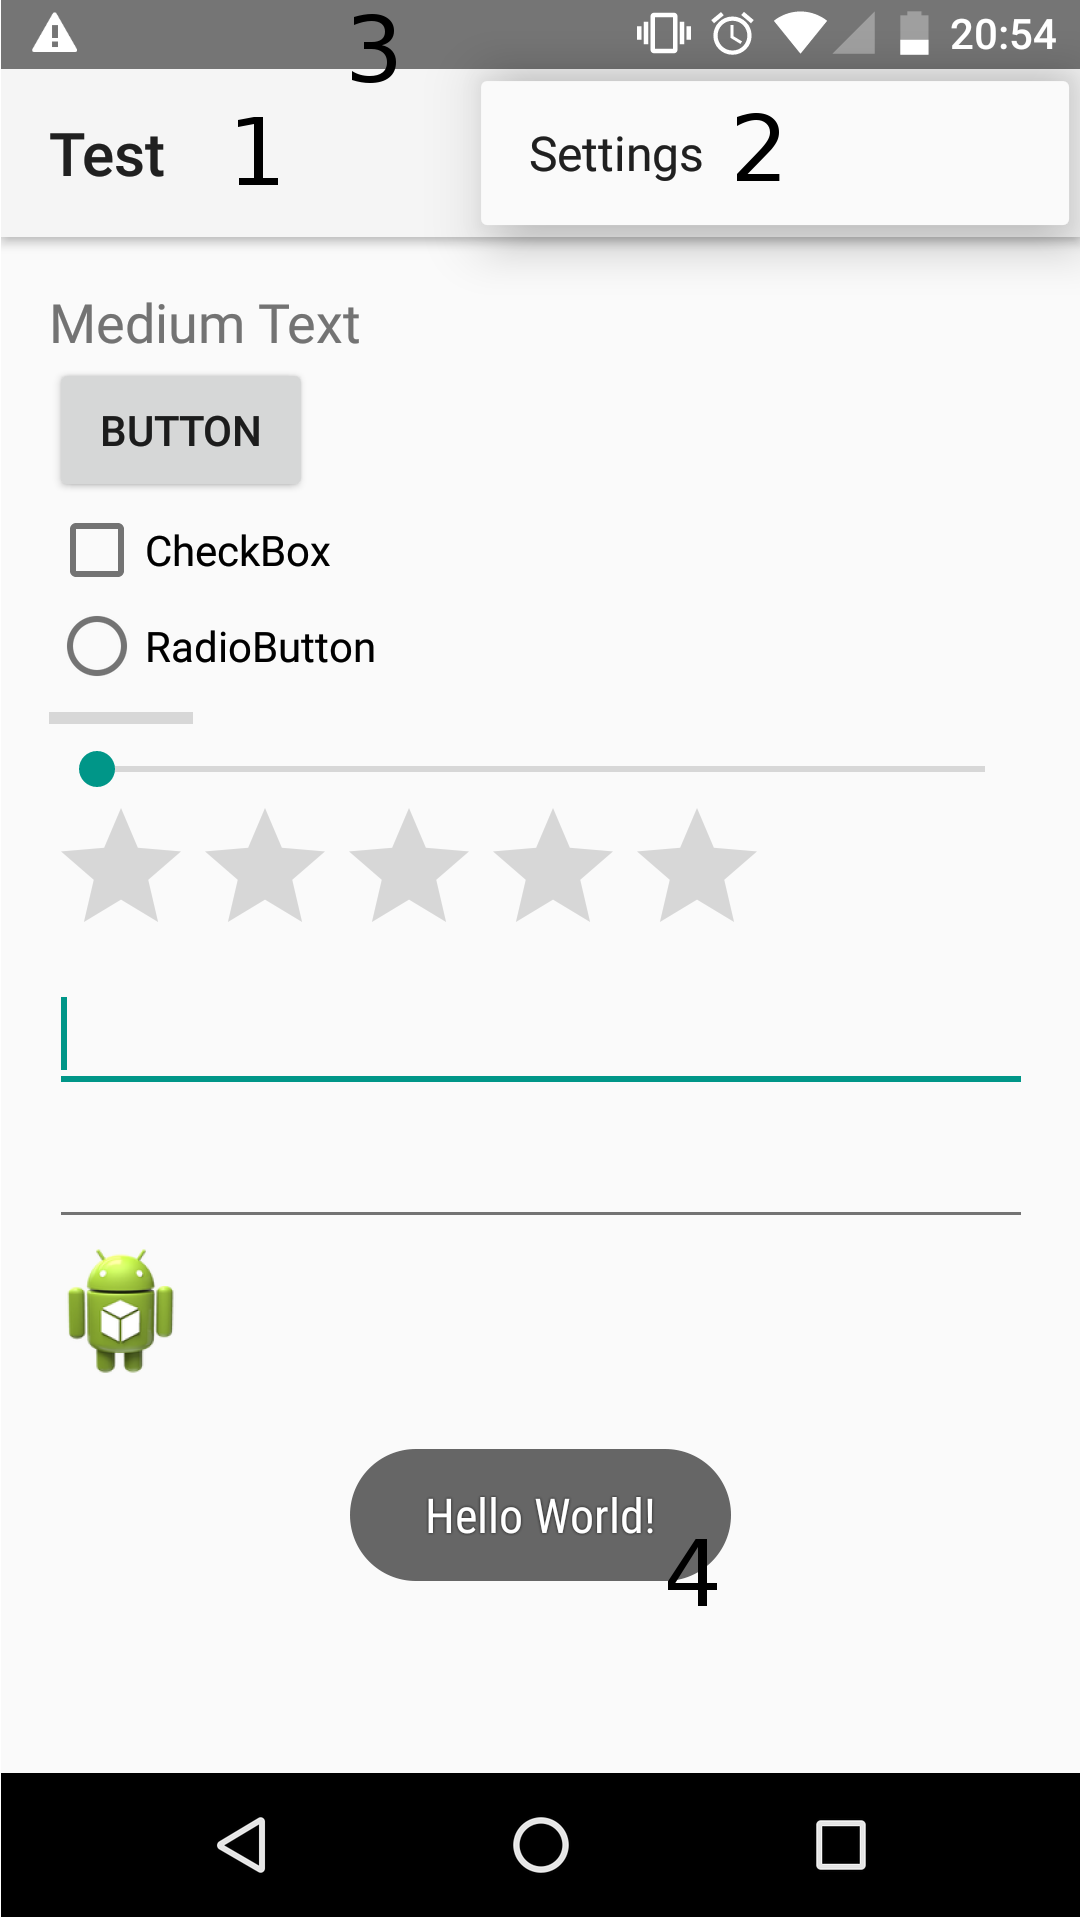
\includegraphics[width=36mm]{img/ui}
		%	\end{picture}
			%\includegraphics[\textwidth]{fig}
		\end{column}
	\end{columns}
}

\subsection{Beschreibung}
\frame{\frametitle{Die Beschreibung des Android UIs}
	\begin{columns}
		\begin{column}{.67\textwidth}
				\tiny {\lstinputlisting[language=XML]{samples/ui2.xml}}
		\end{column}
		
		\begin{column}{.33\textwidth}
			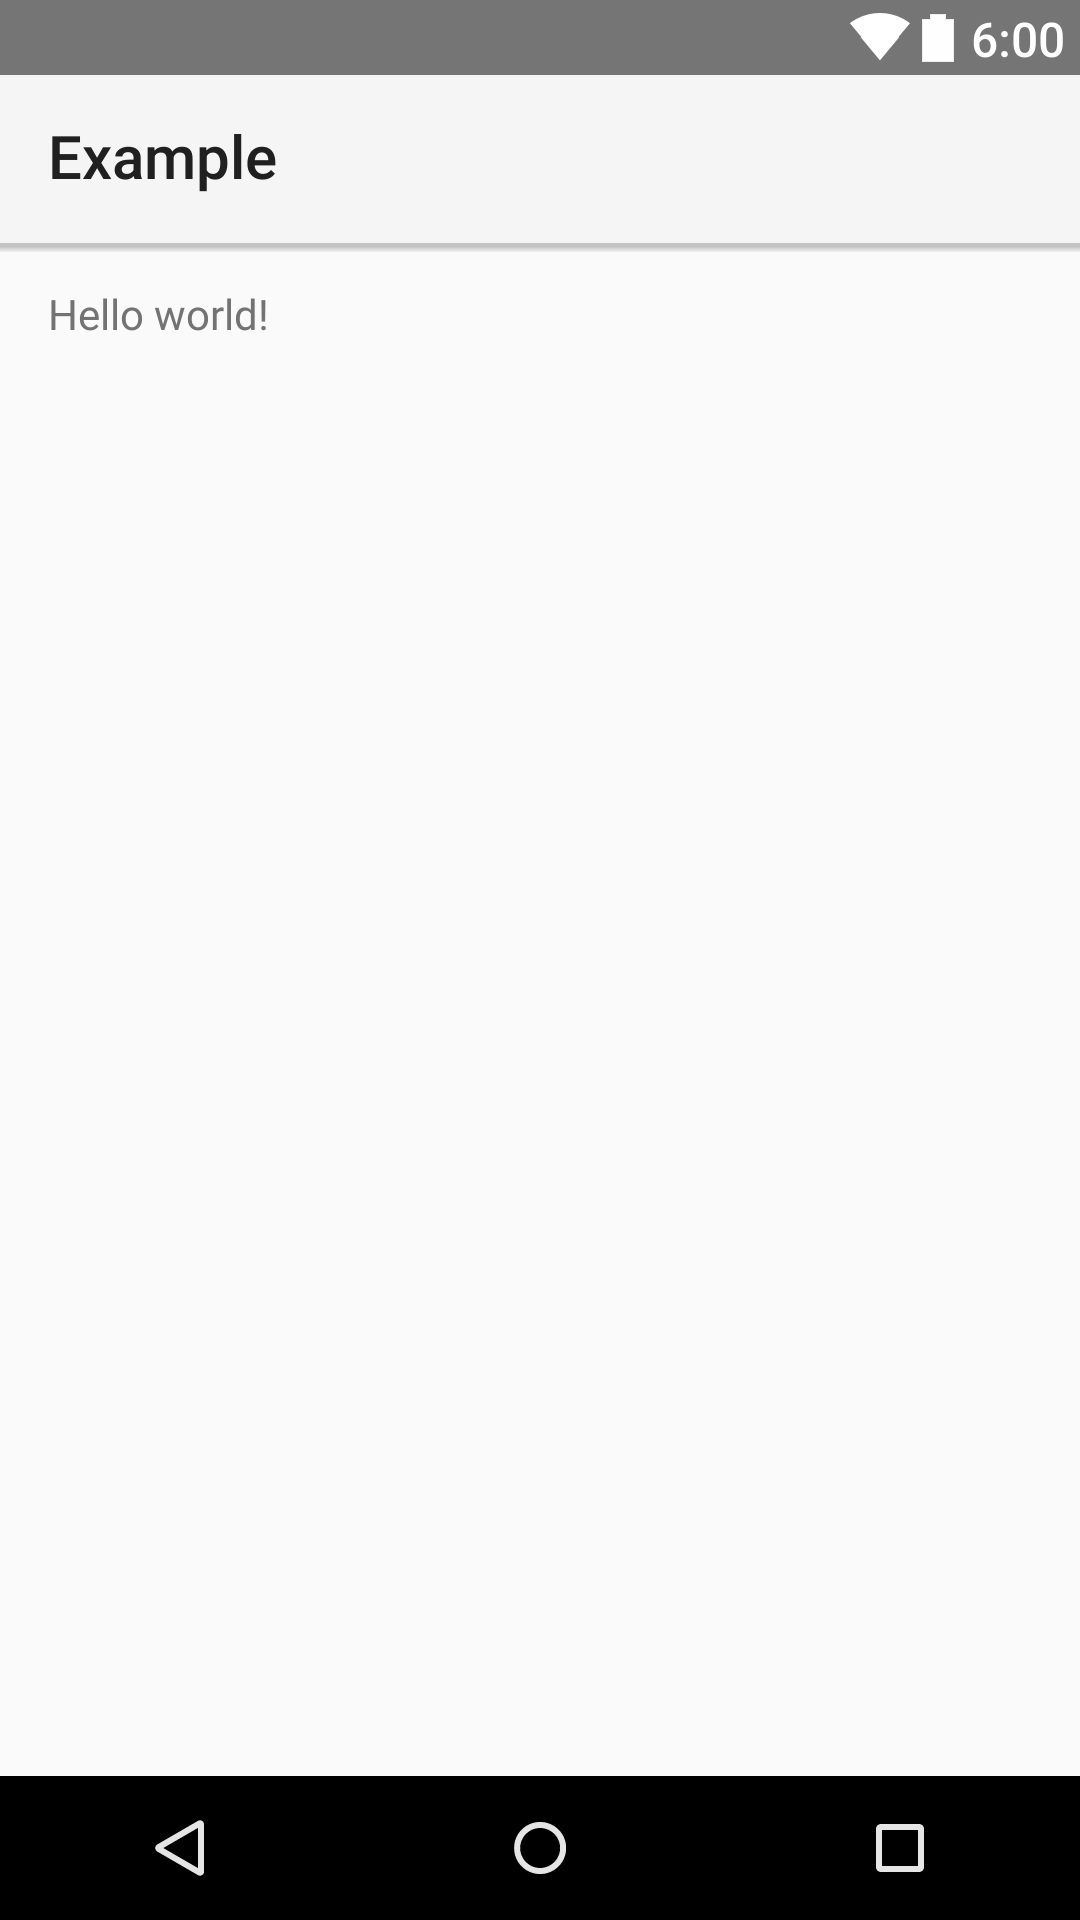
\includegraphics[width=36mm]{img/ui2}
		\end{column}
	\end{columns}
}
\frame{\frametitle{Die Beschreibung des Android UIs}
	\begin{columns}	
		\begin{column}{.67\textwidth}
			\tiny {\lstinputlisting{samples/ui3.xml}}
		\end{column}
		
		\begin{column}{.33\textwidth}
			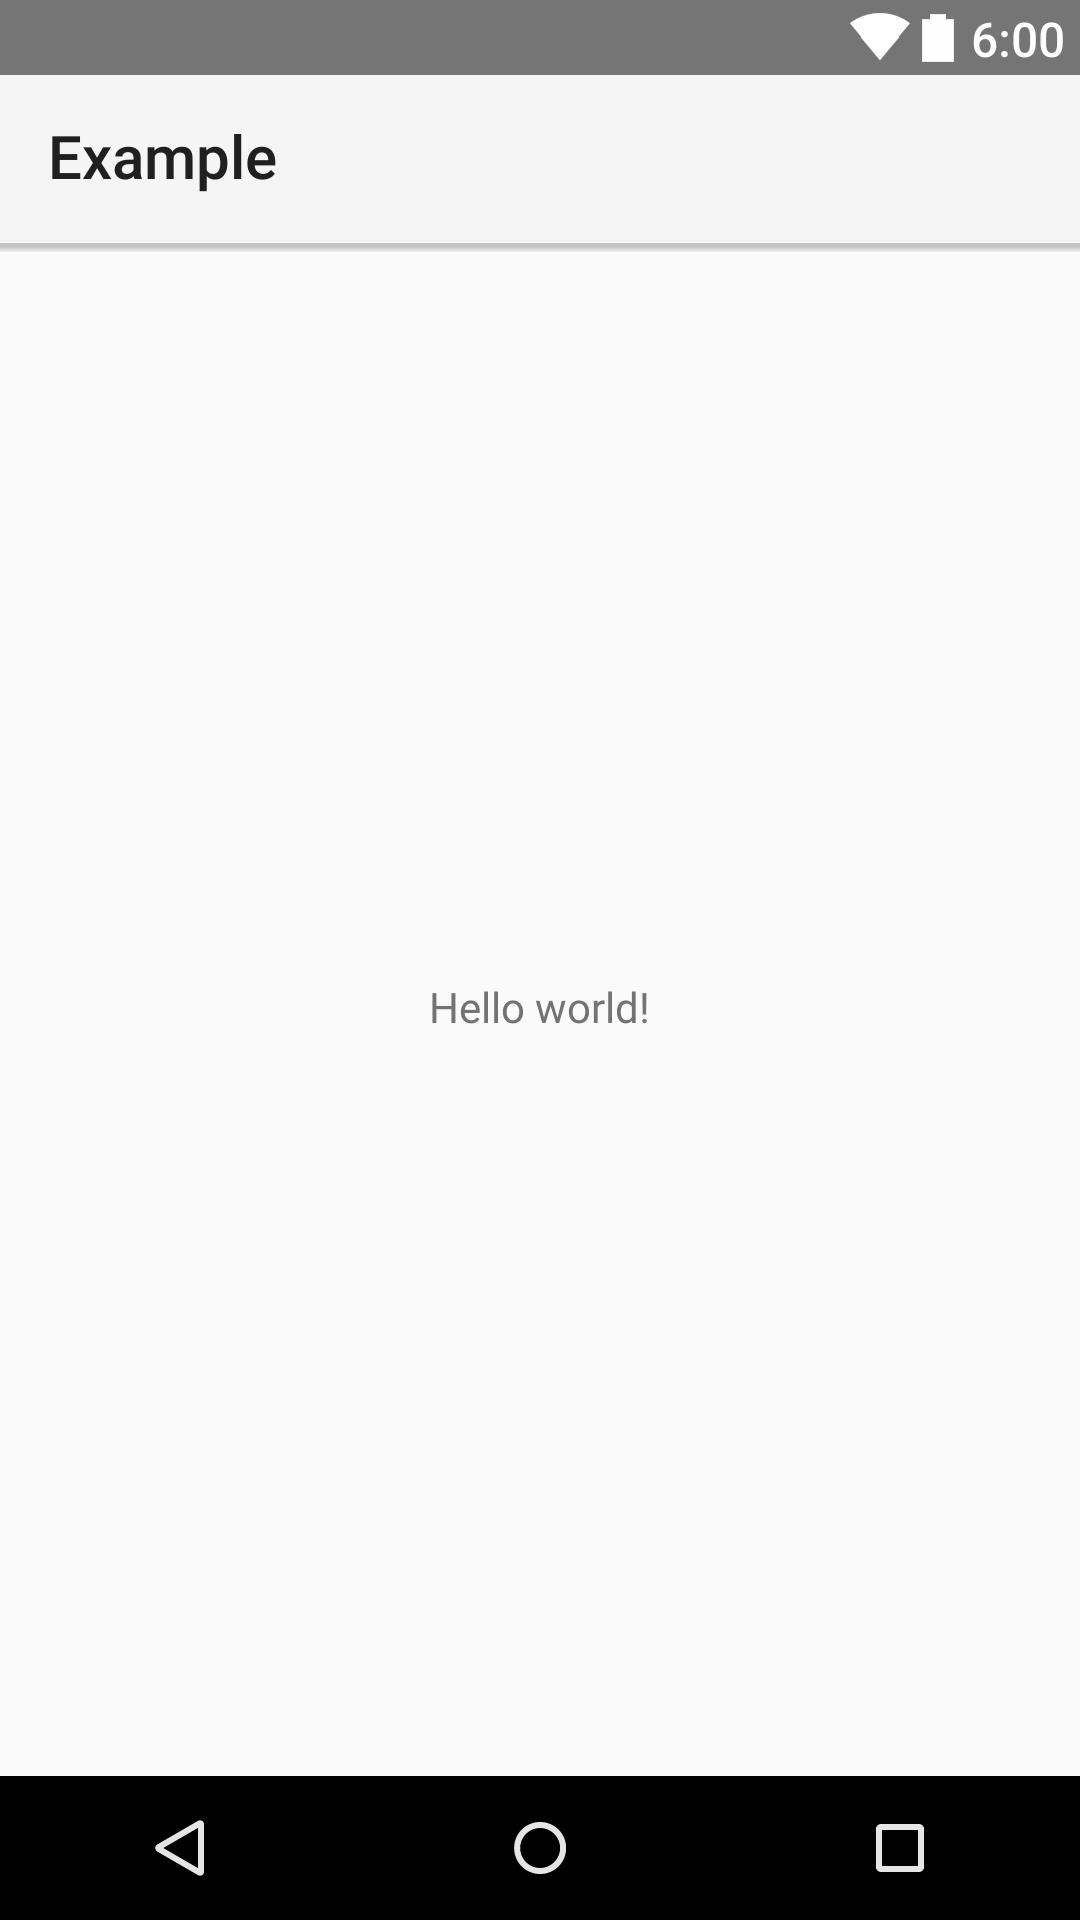
\includegraphics[width=36mm]{img/ui3}
		\end{column}
	\end{columns}
}
\section{UI-Gestaltung}
\forloop{ct}{1}{\value{ct} < 9}%
{%
	\frame{\frametitle{Ein esrtes UI gestalten}		
		\includegraphics[width=116mm]{img/new\arabic{ct}}
	}
}
\section{UI zu Code}
\subsection{Von Android Studio zu NetBeans}
\forloop{ct}{1}{\value{ct} < 6}%
{%
	\frame{\frametitle{Von Android Studio zu NetBeans}		
		\includegraphics[width=116mm]{img/a2n\arabic{ct}}
	}
}
\subsection{Code}
\frame{\frametitle{Vom UI zum Code}
	\begin{itemize}
		\item Jedes UI-Element in Android ist von der Grundklasse ein {\tt View}
		\item Alle UI-Elemente, denen im XML-File eine Id ({\tt android:id=""}) gegeben wurden, werden in Java von der IDE in die Klasse {\tt R} abgebildet
		\item Im Code können die Views dann über {\tt findViewById(R.id.\{viewId\})} referenziert werden
		\item Referenzierung als Button, TextView, usw. der Views im Code durch Casts 
	\end{itemize}
}
\frame{\frametitle{Einen TextView ändern}
	\tiny {\lstinputlisting{samples/MainActivity.java}}
}
\section{Zinsrechner}
\frame{\frametitle{Mini-Projekt: Zinsrechner}
	Designen und Bauen Sie einen kleinen Zinsrechner, bei dem der Benutzer ein Startkapital und einen Zinssatz angeben kann und sein Endkapital zurückgeliefert bekommt.
	
	\pause Musterlösung:\\ \url{https://github.com/janisstreib/RESTaurant/tree/master/Zinsrechner}
}
\section{Zustandshaltung}
\frame{\frametitle{Zustandshaltung}
	\begin{itemize}
		\item Experiment mit dem Zinsrechner: Display drehen (in einem AVD: {\tt Strg + F11} / {\tt Strg + F12}) \pause
		\item Grund: Bei jedem komplett neuen Zeichnen des UIs wird {\tt onCreate()} neu aufgerufen und die Activity neu instanziiert \pause
		\item Lösung: {\tt onSaveInstanceState()} und {\tt onRestoreInstanceState()} sowie der Parameter {\tt savedInstanceState} in {\tt onCreate()}
		\item Variablen und Zustände werden in einem {\tt Bundles} bei {\tt onRestoreInstanceState()} gespeichert und vom Android-System entgegengenommen. Wenn die Activity vom System wieder geweckt wird, wird dieses Bundle der Activity wieder zurückgeführt.
		\item $\Rightarrow$ Android-System kann auch aus anderen Gründen die Activity "killen"
	\end{itemize}
}
\frame{\frametitle{Beispiel}
	\tiny{ \lstinputlisting{samples/Instance.java} }
}
\frame{\frametitle{Implementieren}
	Implementieren Sie die Zustandshaltung in Ihrem Zinsrechner.\\
	Musterlösung: \\\pause
	\url{https://github.com/janisstreib/RESTaurant/tree/master/ZinsrechnerEnhanced}
}
\section{Android Documentaion}
\frame{\frametitle{Android Documentation}
	\begin{itemize}
		\item Aktuelle Guidelines, Tutorials, Dokumentation: \\ \url{https://developer.android.com}
	\end{itemize}
}
%\section{Teil IV: Android UI-Design}
%\section{Teil V: Das RESTAurant}
%\section{Optional: Teil VI: Android Design Guidelines}
%\section{Optional: Teil VII: Versionskontrolle}
\end{document}


	\part{Teil IV}
	\documentclass{beamer}
\usepackage[utf8]{inputenc}
\usepackage{hyperref}
\usepackage{forloop}
\usepackage{amsmath,amsfonts,amssymb}
\useoutertheme {smoothbars}
\usepackage{verbatim}
\usepackage{listings}
\usepackage{color}
\definecolor{name}{rgb}{0.5,0.5,0.5}
\definecolor{javared}{rgb}{0.6,0,0} % for strings
\definecolor{javagreen}{rgb}{0.25,0.5,0.35} % comments
\definecolor{javapurple}{rgb}{0.5,0,0.35} % keywords
\definecolor{javadocblue}{rgb}{0.25,0.35,0.75} % javadoc

\lstset{language=Java,
	basicstyle=\ttfamily,
	keywordstyle=\color{javapurple}\bfseries,
	stringstyle=\color{javared},
	commentstyle=\color{javagreen},
	morecomment=[s][\color{javadocblue}]{/**}{*/},
	numbers=left,
	numberstyle=\tiny\color{black},
	stepnumber=2,
	numbersep=10pt,
	tabsize=4,
	showspaces=false,
	showstringspaces=false}

\defbeamertemplate*{footline}{smoothbars theme}
{%
	\begin{beamercolorbox}[colsep=1.5pt]{upper separation line foot}
	\end{beamercolorbox}
	\begin{beamercolorbox}[ht=2.5ex,dp=1.125ex,%
		leftskip=.3cm,rightskip=.3cm plus1fil]{title in head/foot}%
		\leavevmode{\usebeamerfont{title in head/foot}\insertshorttitle}%
		\hfill%
		{\usebeamerfont{author in head/foot}\usebeamercolor[fg]{author in head/foot}\insertshortauthor}%
	\end{beamercolorbox}%
	\begin{beamercolorbox}[colsep=1.5pt]{lower separation line foot}
	\end{beamercolorbox}
}

\begin{document}

\title{RESTaurant for Android: Programmierung einer Sitzplatzreservierung \\ Teil IV}   
\author{Janis Streib \\ CC-BY-SA} 
\date{02.-06.11.2015} 

\frame{\titlepage} 

\frame{\frametitle{Inhalt}\tableofcontents} 

%\lstinputlisting{filename.java}
%\begin{lstlisting}
% Add code here
%\end{lstlisting}
\section{RESTaurant?}
\subsection{REST}
\frame{\frametitle{REST}
	\begin{itemize}
		\item Der RESTaurant-Server bietet zur Kommunikatoin mit der App ein REST-API über http an
		\item API := Application Programming Interface
		\item REST (oder ReST) := Representational State Transfer
		\item "REST fordert, dass eine URI (Adresse) genau einen Seiteninhalt repräsentiert, und dass ein Web-/REST-Server auf mehrfache Anfragen mit demselben URI auch mit demselben Webseiteninhalt antwortet." - \url{https://de.wikipedia.org/wiki/Representational_State_Transfer}
	\end{itemize}
}
\subsection{JSON}
\frame{\frametitle{JSON}
	\begin{columns}
		\begin{column}{0.727\textwidth}
	\begin{itemize}
		\item JSON := JavaScript Object Notation
		\item Einfach lesbares Textformat
		\item Array: \\ {\tt ["hallo1", "hallo2"]}
		\item Object: \\ {\tt \{\\\hspace{1ex}	"EventType": "Workshop",\\\hspace{1ex}	"Teacher": "Janis Streib",\\\hspace{1ex} "Participants": 5\\\}}
		\item In Java: org.json-Library\\\url{http://www.json.org/java/index.html}
	\end{itemize}
\end{column}
\begin{column}{0.373\textwidth}
	\pause
	
\includegraphics[width=40mm]{img/REST}
\end{column}
\end{columns}
}
\subsection{HTTP}
\frame{\frametitle{HTTP}
	Beispiel eines HTTP-GET-Requestes an einen Webserver auf www.dogcraft.de:
	{\tiny \verbatiminput{samples/http.txt}}
}
%\section{Teil V: Das RESTAurant}
%\section{Optional: Teil VI: Android Design Guidelines}
%\section{Optional: Teil VII: Versionskontrolle}
\end{document}


\end{document}